\emph{\textbf{Scenario}}

Lorenzo is a student who is living in Rome. During the summer, he decides to go on a trip to Milan. Due to the fact that Milan is a really crowded city and number of accidents and traffic violations have skyrocketed in the recent decade, he is skeptical to drive his personal car to enjoy the eye-catching scenery along the way or book a flight. His friend suggests to use the SafeStreets app to check the safety of the area he will be staying in Milan in order to decide whether it would be safe to leave his car behind and move on foot there. He opens the app searches for the area his hotel is in and views the safety of nearby streets.

\emph{\textbf{Use Case}}

\begin{table}[!hbtp]
\footnotesize
\centering
\settowidth\tymin{\textbf{Name}}
\setlength\extrarowheight{2pt}
\begin{tabulary}{\textwidth}{|J|J|}
\hline
Name  & View Safety \\
\hline
Actor & Registered User \\
\hline
Entry conditions & The user wants to check the safety of a certain area that he is interested in \\
\hline
Events flow & 
\begin{minipage}[t]{0.7\textwidth}
\begin{enumerate} 
\item In the homepage the user opens the view safety section of the app
\item The user specifies details of the area he is interested in
\item The user submits search criteria and chooses area from a list of matches
\item The user is represented with a geographical representation of the area’s safety based on number of violations and accidents occurring in the area
\end{enumerate}
\end{minipage}\\
\hline
Exit conditions  & The user is represented with area safety\\
\hline
Exceptions       & 
\begin{minipage}[t]{0.8\textwidth}
\begin{itemize} 
\item The specified area does not yield any search results: A message stating there are no results matching entered data is shown
\end{itemize}
\end{minipage}\\
\hline
\end{tabulary}
\caption{\label{tab:xx}xx}
\end{table}

\emph{\textbf{Sequence Diagram}}

\begin{figure}[H]
\caption{Sequence diagram for Login}
\label{fig:SD-login}
\centering
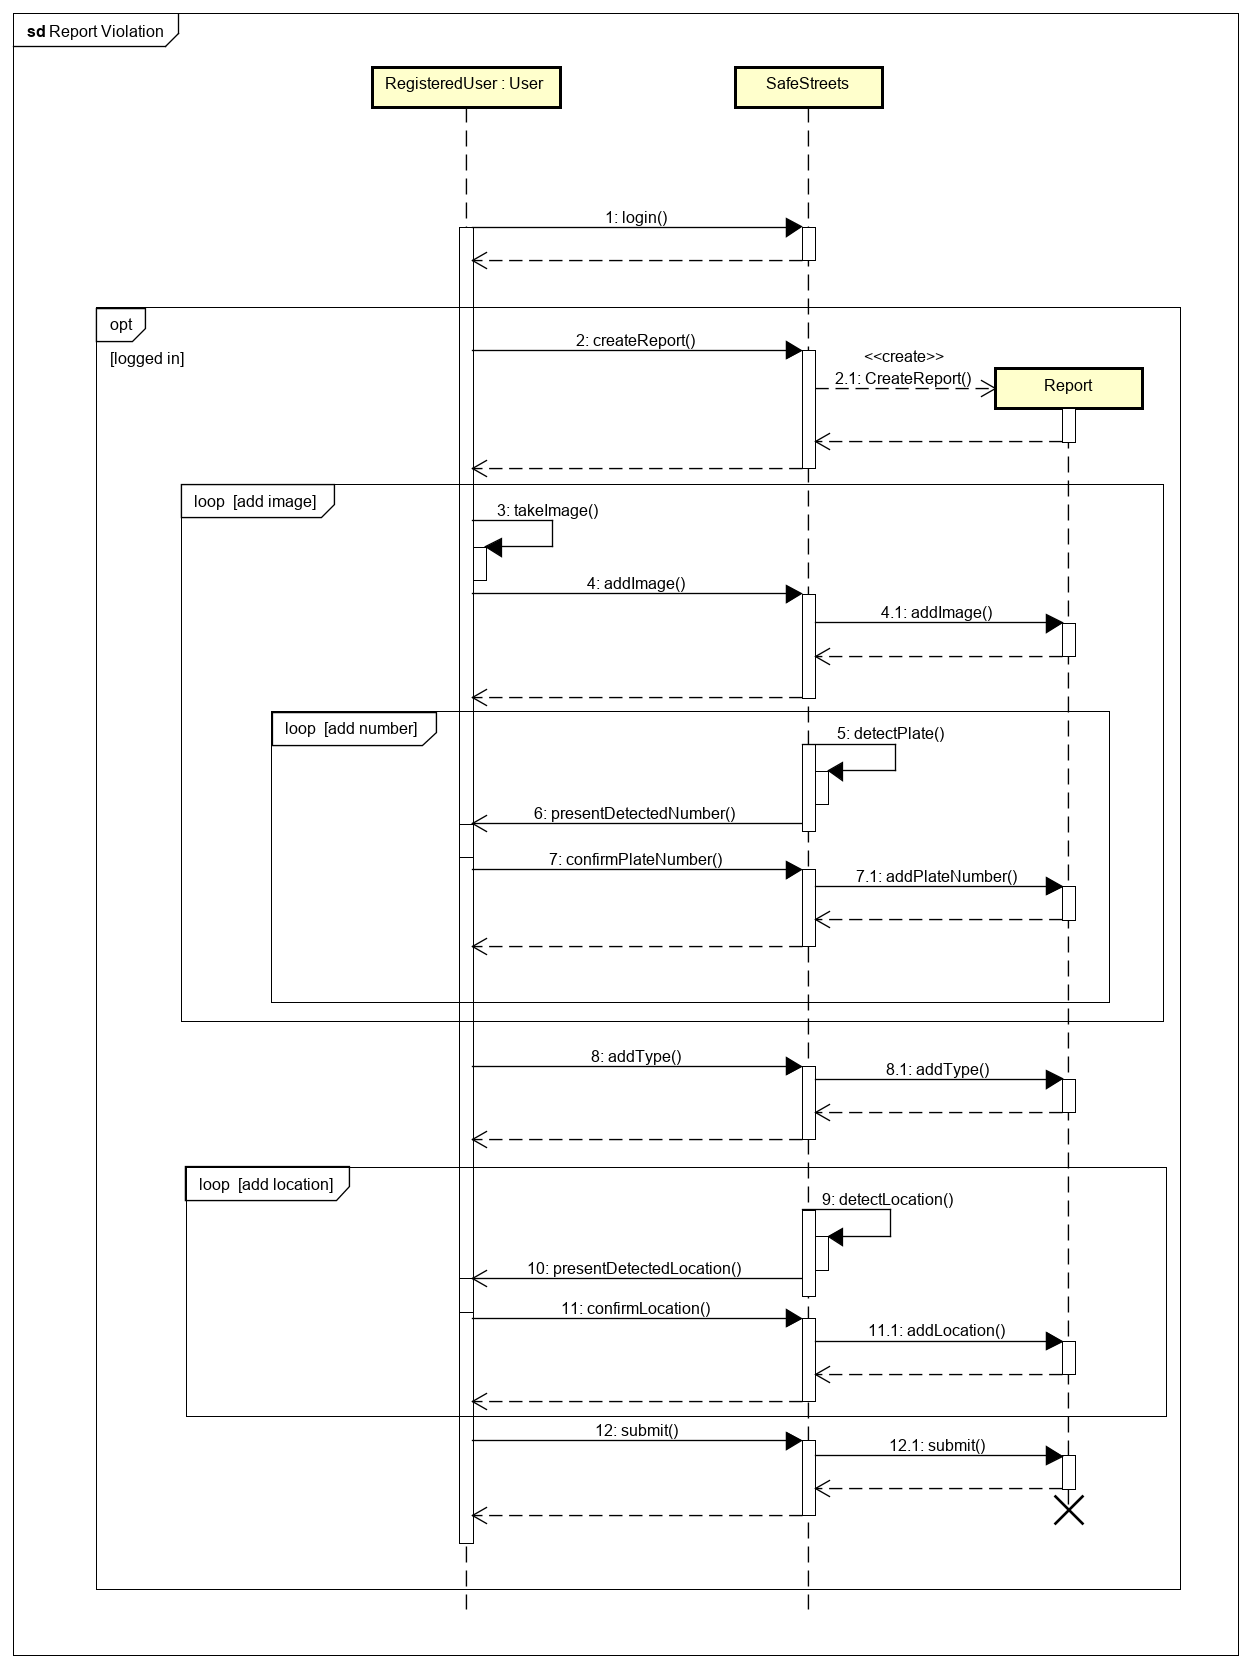
\includegraphics[width=\textwidth, height=\textheight]{report-violation-SD.png}
\end{figure}


%***place holder for report-violation-sd***
